% % % % % % % % % % % % % % % % % % % % % % % % % % % % % % % % % % % % % % % % % % % %
%                                                                                     %
% Short Sectioned Assignment LaTeX Template Version 1.0 (5/5/12)                      %
% This template has been downloaded from: http://www.LaTeXTemplates.com               %
%                                                                                     %
% Original author:  Frits Wenneker (http://www.howtotex.com)                          %
%                                                                                     %
% Modified by: Fco Javier Sueza Rodríguez (fcosueza@disroot.org)                      %
%                                                                                     %
% Changes:                                                                            %
%	    - Custom Chapters, Sections and Subsections (titlesec package)                %
%           - Document type scrbook (oneside)                                         %
%           - Use babel-lang-spanish package and marvosym                             %
%           - Use hyperref, enumitem, tcolorbox and glossaries packages               %
%           - Use Time New Roman (mathptmx), Helvetic and Courier fonts               %
%                                                                                     %
% License: CC BY-NC-SA 3.0 (http://creativecommons.org/licenses/by-nc-sa/3.0/)        %
%                                                                                     %
% % % % % % % % % % % % % % % % % % % % % % % % % % % % % % % % % % % % % % % % % % % %

%-----------------------------------------------%
%	              Packages                  %
%-----------------------------------------------%

\documentclass[paper=a4, fontsize=11pt, oneside]{scrbook}

% ---- Text Input/Output ----- %

\usepackage[T1]{fontenc}
\usepackage[utf8]{inputenc}
\usepackage{mathptmx}
\usepackage[scaled=.92]{helvet}
\usepackage{courier}
\usepackage[indent=12pt]{parskip}

\usepackage{geometry}
\geometry{verbose,tmargin=3cm,bmargin=3cm,lmargin=2.6cm,rmargin=2.6cm}

% ---- Language ----- %

\usepackage[spanish]{babel}
\usepackage{marvosym}

% ---- Another packages ---- %

\usepackage{amsmath,amsfonts,amsthm}
\usepackage{graphics,graphicx}
\usepackage{titlesec}
\usepackage{fancyhdr}
\usepackage{tcolorbox}
\usepackage{hyperref}
\usepackage{enumitem}
\usepackage[automake]{glossaries}

%--------------------------------------------------------------------%
%                      Customizing Document                          %
%--------------------------------------------------------------------%


% ----------- Custom Chapters, Sections and Subsections -------------- %

\titleformat{\chapter}[display]
			{\bfseries\Huge}
			{Tema \ \thechapter} {0.5ex}
			{\vspace{1ex}\centering}

\titleformat{\section}[hang]
			{\bfseries\Large}
			{\thesection}{0.5em}{}

\titleformat{\subsection}[hang]
			{\bfseries\large}
			{\thesubsection}{0.5em}{}

\titleformat{\subsubsection}[hang]
			{\bfseries\large}
			{\thesubsubsection}{0.5em}{}

\hypersetup{
    colorlinks=true,
    linkcolor=black,
    urlcolor=magenta
}

% ------------------- Custom heaaders and footers ------------------- %

\pagestyle{fancyplain}

\fancyhead[]{}
\fancyfoot[L]{}
\fancyfoot[C]{}
\fancyfoot[R]{\thepage}

\renewcommand{\headrulewidth}{0pt} % Remove header underlines
\renewcommand{\footrulewidth}{0pt} % Remove footer underlines

\setlength{\headheight}{13.6pt} % Customize the height of the header

% --------- Numbering equations, figures and tables ----------------- %

\numberwithin{equation}{section} % Number equations within sections
\numberwithin{figure}{section} % Number figures within sections
\numberwithin{table}{section} % Number tables within sections

% ------------------------ New Commands ----------------------------- %

\newcommand{\horrule}[1]{\rule{\linewidth}{#1}} % Create horizontal rule command


%----------------------------------------------------------------------------------------
%	TÍTULO Y DATOS DEL ALUMNO
%----------------------------------------------------------------------------------------

\title{
\vspace{10ex}
\normalfont \normalsize
\huge \textbf{Documentación y Control de Versiones}
}
\author{Francisco Javier Sueza Rodríguez}
\date{\normalsize\today}

%----------------------------------------------------------------------------------------
%                                     DOCUMENTO
%----------------------------------------------------------------------------------------
\begin{document}


\maketitle

\thispagestyle{empty}

\vspace{65ex}

\begin{center}
    \begin{tabular}{l l}
        \textbf{Centro}: & IES Aguadulce \\
        \textbf{Ciclo Formativo}: & Desarrollo Aplicaciones Web (Distancia)\\
        \textbf{Asignatura}: & Despliegue de Aplicaciones Web\\
        \textbf{Tema}: & Tema 5 - Documentación y Control de Versiones\\
    \end{tabular}
\end{center}

\newpage

\tableofcontents

\newpage

\section{Actividad 1: phpDocumentor}
Este ejercicio relacionado con generación de documentación consistirá en los siguientes apartados :

\subsection{Actividad 1.1}
Instala la herramienta phpdocumentor en tu servidor Linux y comenta los aspectos más importantes de tal herramienta, así como las etiquetas principales que se usan.

\subsubsection{Solución}
En este ejercicio vamos a realizar la instalación de \textbf{phpDocumentor} en la distribución \textbf{Kubuntu 22.04} de Linux. Hay varios métodos para realizar la instalación, se puede hacer mediante \textbf{Docker}, usando \textbf{Phive} o \textbf{manualmente}. La instalación mediante composer no es recomendada por los desarrolladores de phpDocumentor, ya que hay una alta probabilidad de que se generen conflictos con otras librerías.

Nosotros hemos optado por la \textbf{opción de instalación manual}. Para ello, solo hemos tenido que descargar el \textbf{paquete de phpDocumentor} del repositorio de \href{https://github.com/phpDocumentor/phpDocumentor/releases}{repositorio de Github} de la aplicación, desde donde hemos descargado la \textbf{versión 3.4.3}.

Una vez descargada la versión simplemente le hemos \textbf{agregado permisos de ejecución} y la hemos movido al directorio \textit{/usr/local/bin}, para que se puede ejecutar desde cualquier parte del sistema, como podemos ver en la siguiente captura.

\begin{figure}[H]
\centering
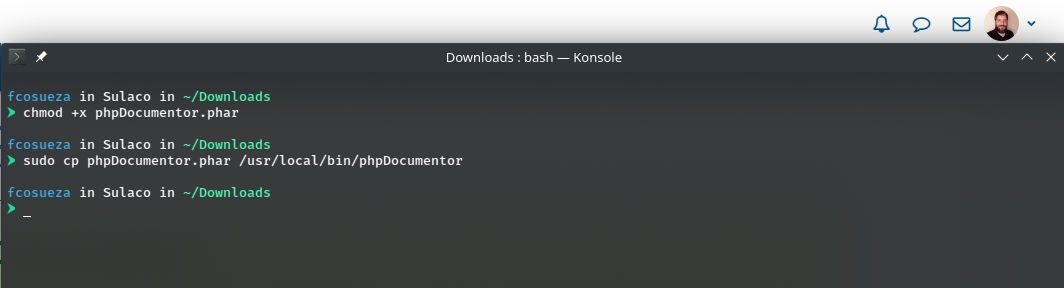
\includegraphics[scale=0.50]{installDoc.png}
\end{figure}

Actualmente, \textbf{phpDocumentor} es la aplicación más empleada para le \textbf{generación de documentación} en aplicaciones desarrolladas con PHP. Es el equivalente para PHP de \textbf{JavaDoc} para Java. Su instalación, como hemos visto, se hace de forma muy sencilla y su uso es igualmente sencillo, pudiendo ejecutarse desde la \textbf{línea de comandos}, la \textbf{interfaz web} o desde el \textbf{propio código PHP}.

Esta aplicación esta desarrollada en PHP y usa el lenguaje para la generación de la documentación, empleando para ello los \textbf{DocBlocks}, que son trozos de código incluidos en el código PHP que sirven para describir la funcionalidad, parámetros, valores devueltos, etc.., de una función, constante, propiedad, etc.

Además, phpDocumentator nos permite generar la documentación en una \textbf{variedad de formatos}, entre los se incluyen \textbf{HTML}, \textbf{PDF} y \textbf{XML}. Esta última opción es muy interesante, ya que mediante el uso de XSL podemos realizar transformaciones sobre el documento, extraer información, etc.

Dentro de los DocBlocks podemos usar un \textbf{conjunto de etiquetas} para describir diferentes elementos de la función que estamos documentando, siendo las más empleadas las siguientes:

\begin{itemize}
    \item \textbf{@package}: se empleada para añadir documentación general en un fichero a nivel de clase.
    \item \textbf{@access}: se usa para especificar si se va a generar o no la documentación de un elemento concreto. En caso de que no queramos que esta genere, por ejemplo, porque es un método privado, podemos indicarle el valor \textbf{\textit{private}}, con lo que la documentación de ese elemento no se generará.
    \item \textbf{@author}: se emplea para indicar el autor de código.
    \item \textbf{@copyright}: indicar información sobre los derechos de uso del elemento.
    \item \textbf{@deprecated}: se usa para indicar que un elemento ha sido deprecado y que no debería usarse.
    \item \textbf{@internal}: se usa para incluir documentación que solo estará disponible para los desarrolladores.
    \item \textbf{@link}: incluye un enlace a un recurso.
    \item \textbf{@see}: se usa para crear un enlace interno a un elemento, por norma general relacionado con el elemento que se esta
    documentando.
    \item \textbf{@version}: indica la versión del elemento.
    \item \textbf{@global}: se usa para especificar variables globales dentro de una función.
    \item \textbf{@param}: describe los parámetros que recibe una función.
    \item \textbf{@return}: describe el valor devuelve por una función.
\end{itemize}

Como podemos ver, para aquel que este familiarizado con JavaDoc todo esto ya le sonará, ya que las similitudes son muchas e incluso la sintaxis que se emplea es prácticamente la misma.

\subsection{Actividad 1.2}
En esta actividad debes crear en tu servidor un script PHP con el nombre practica-XXXXXX.php, donde XXXXXX será tu apellido. A continuación escribe dentro de este script bloques de código y DocBlocks para que luego se pueda generar la documentación correspondiente. El script debe contener al menos dos funciones documentadas, indicando mediante las etiquetas vistas en la unidad los siguientes elementos:

\begin{itemize}
    \item Parámetros de entrada de la función.
    \item Parámetros de devuelve la función.
    \item Autor y versión del script.
    \item Una anotación que solo sea visible en la documentación para desarrolladores.
\end{itemize}

\subsubsection{Solución}
En este ejercicio se ha creado un script, \textbf{\textit{practica-SUEZA.php}}, que genera un mensaje sencillo y procesa una fecha indicando la fecha actual. El script se adjunta con el trabajo por lo que no vamos a entrar en detalles sobre éste.

Una vez creado el script, se ha usado \textbf{phpDocumentor} para generar la documentación empleando para ello el comando \textbf{\textit{phpDocumentor -run -d . -t docs/}}, donde se le indica que el directorio donde tiene que el actual y que la documentación generada la almacene en el directorio \textbf{\textit{docs}}.

En la siguiente captura, vemos la ejecución de phpDocumentor y la estructura de directorios que ha generado en el proceso.

\begin{figure}[H]
    \centering
    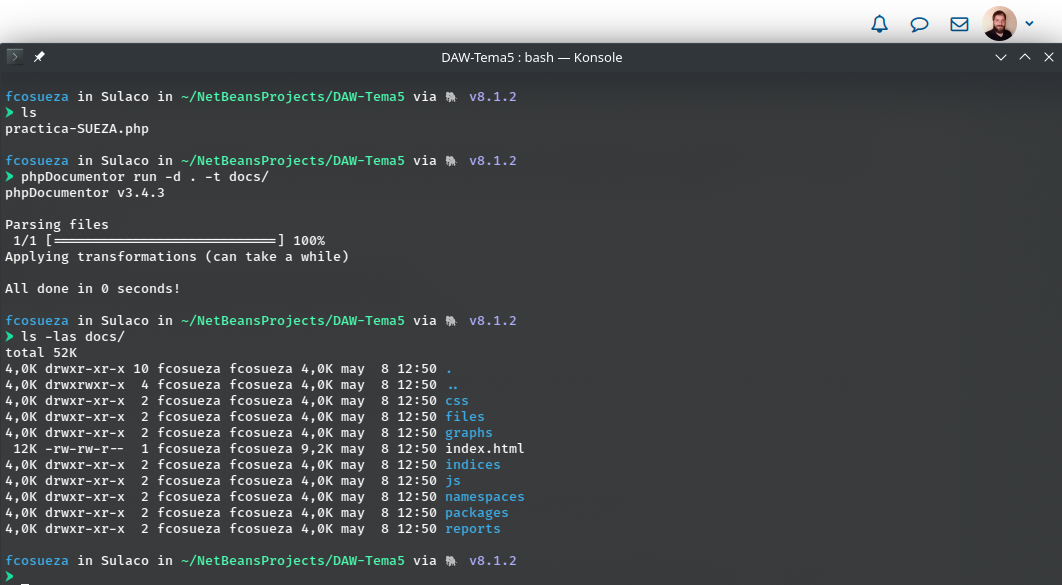
\includegraphics[scale=0.50]{genDoc.png}
\end{figure}

Como podemos ver, se ha generado una estructura de directorios donde se almacenan diferentes elementos, en este caso que la salida ha sido en \textbf{HTML}, hay archivos de estilo CSS, archivos Javascript, etc...

En la siguiente captura, podemos ver la visualización del archivo principal de la documentación en una navegador.

\begin{figure}[H]
    \centering
    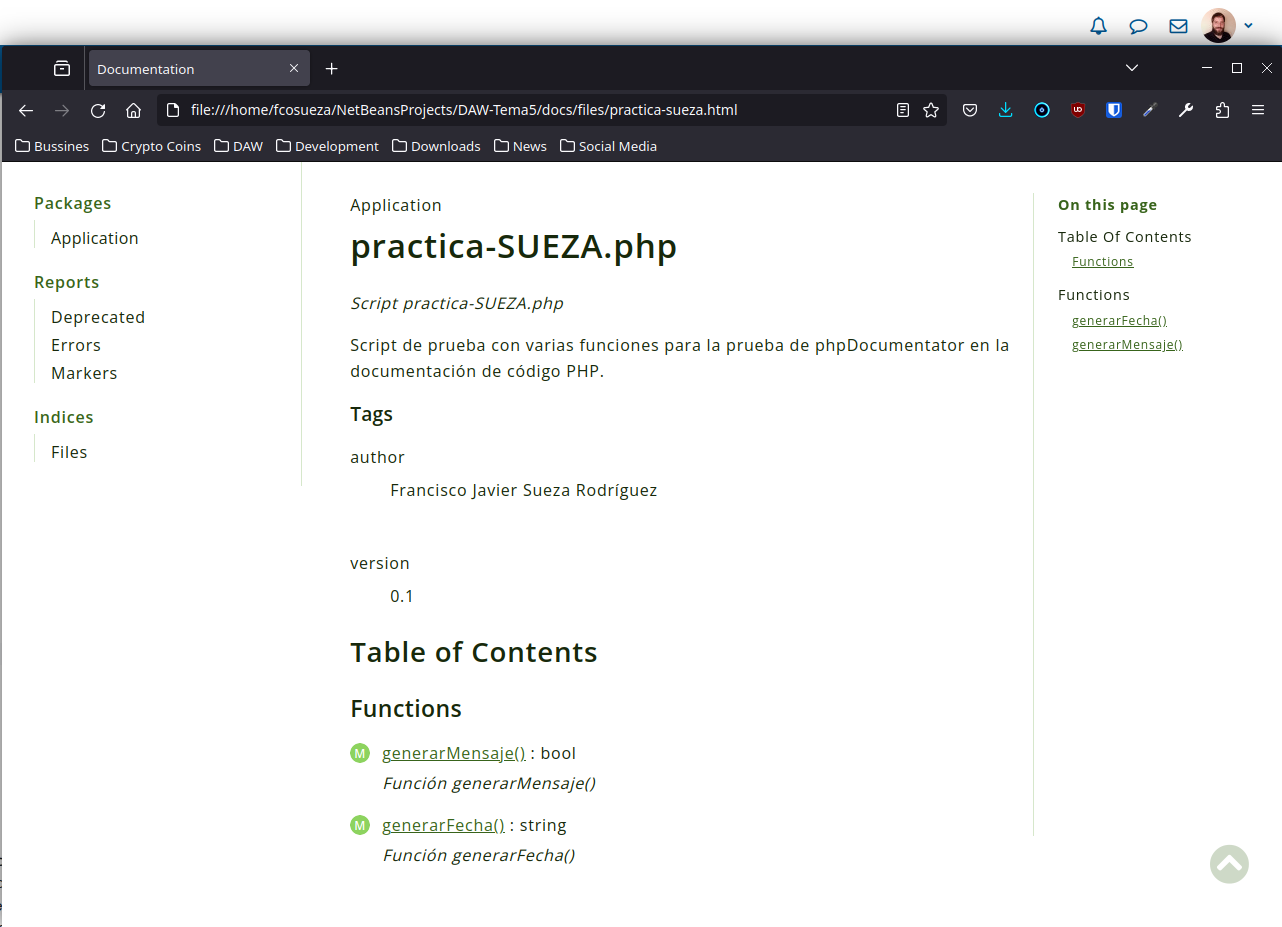
\includegraphics[scale=0.40]{viewDoc.png}
\end{figure}

\section{Ejercicio 2: Git y GitHub}
Este ejercicio está relacionado con \textbf{Github}, se puede realizar en Windows, que consistirá en los siguientes apartados.

\subsection{Ejercicio 2.1}
Elabora un pequeño tutorial donde será necesario instalar git en Windows y configurarlo en tu computadora, donde se detallarán las explicaciones teóricas (¿Qué es Git? ¿Para qué sirve? ¿Última versión? etc..)y las capturas de pantallas que sean necesarias.


\subsubsection{Solución}
\textbf{Git} es un software de \textbf{control de versiones}  de versiones desarrollado por \textbf{Linus Torvalds} en 2005 como sustituto para Bitkeeper para el control del código del kernel de Linux. Desde entonces, se ha popularizado y es sistema de control de versiones más extendido en el desarrollo de aplicaciones.

Algunas de las principales características de Git son las siguientes:

\begin{itemize}
    \item Buen \textbf{soporte} para el \textbf{desarrollo no lineal}, permitiendo la creación de ramas y su mergeado rápidamente, así como herramientas para la navegación sobre el historial de cambios.
    \item Es un \textbf{sistema distribuido}. Cada desarrollador tiene una copia local del repositorio y los cambios se van propagando entre estos repositorios locales, agrupando los cambios en ramas y mergeándolos a la rama principal.
    \item Los \textbf{repositorios} pueden ser \textbf{publicados} empleando protocolos existentes como \textbf{HTTP}, \textbf{HTTPS}, \textbf{FTP} o \textbf{SSH}.
    \item Es \textbf{muy eficiente} en el \textbf{manejo de proyectos grandes}, siendo muy rápido y escalable.
    \item Permite \textbf{autenticación criptográfica del historial} de cambios.
\end{itemize}

Actualmente, la \textbf{última versión} de Git es la \textbf{2.45.0} que fue lanzada el \textbf{29 de Abril de 2024}, y este puede ser instalados la mayoría de sistemas operativos, entre los que nos encontramos \textbf{Linux}, \textbf{Windows}, \textbf{MacOS} o \textbf{Solaris}.

En nuestro caso, vamos a realizar su instalación en una \textbf{Kubuntu 22.04}, ya que Linux es uno de los sistemas operativos más empleado para el desarrollo de aplicaciones y uno de los que mejor integra Git.

Para realizar la \textbf{instalación y configuración} de Git en Linux vamos a usar el gestor de paquetes \textbf{APT} para instalar la aplicación, empleando para ello el comando \textbf{\textit{apt-get install git}}, lo cual no solo nos realizará la instalación sino que nos dejará la aplicación con una configuración inicial lista para ser usada. En la siguiente captura podemos ver la ejecución de este comando en la consola de Linux.

    \begin{figure}[H]
        \centering
        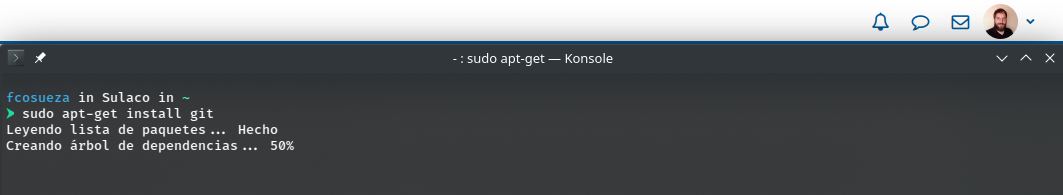
\includegraphics[scale=0.50]{gitInstall.png}
    \end{figure}


\subsection{Ejercicio 2.2}
Realiza la siguiente configuración:

\begin{itemize}
    \item Configura tu nombre, apellidos y cuenta de correo
    \item Muestra la versión instalada.
    \item Indica cuál es tu directorio de trabajo.
\end{itemize}

\subsubsection{Solución}
Una vez realizada la instalación de Git, vamos a realizar una configuración básica y a mostrar información sobre la versión instalada y el directorio de trabajo.

\begin{enumerate}
    \item Primero vamos a configurar \textbf{nuestro usuario y correo electrónico}. Aunque se puede hacer de forma global, es recomendable hacerlo de forma local al usuario con el que vamos a usar Git. Para ello, debemos podemos crear el fichero \textbf{\textit{.gitconfig}} en nuestro \textbf{directorio Home} y añadir la información del usuario y el correo como vemos en la siguiente captura.

    \begin{figure}[H]
        \centering
        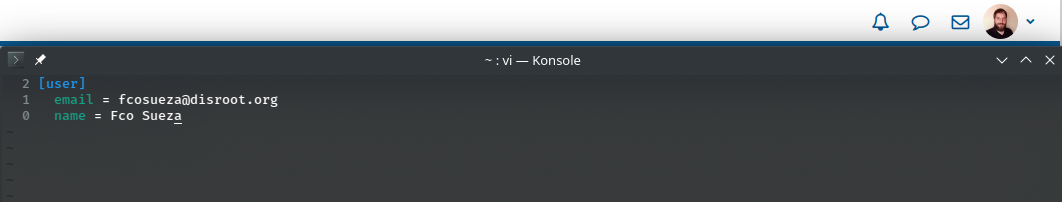
\includegraphics[scale=0.50]{gitConfig.png}
    \end{figure}

    \item A continuación, podemos emplear el comando \textbf{\textit{git --version}} para comprobar que la instalación se ha realizado correctamente y que versión es la que se instalado. En nuestro caso ha sido la \textbf{versión 2.34.1}, que no es la última versión de la aplicación ya que se ha descargado de los repositorios de Kubuntu y a veces tardan un poco en incluir las nuevas versiones en las ramas estables de la distribución.

    \begin{figure}[H]
        \centering
        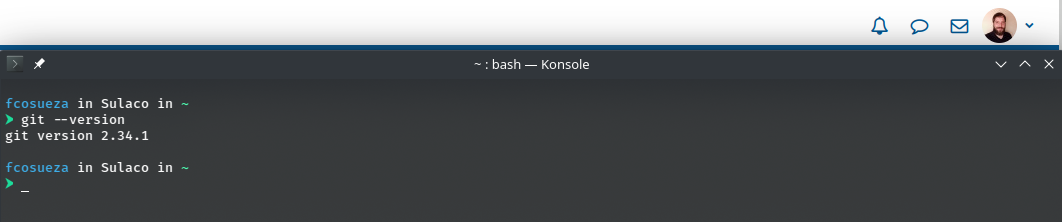
\includegraphics[scale=0.50]{gitVersion.png}
    \end{figure}

    \item Ya tenemos git instalado y configurado. Ahora vamos a \textbf{crear un repositorio} en el proyecto PHP del apartado anterior. en nuestro caso el proyecto solo tiene un archivo PHP y la documentación generada con phpDocumentor.

    Para crear el repositorio, usamos el comando \textbf{\textit{git init}}, que creará el repositorio git generando el directorio .git con toda la información del repositorio, como el indice, los objetos, las ramas que tiene, etc.

    En la siguiente captura, podemos ver la creación del repositorio, donde además se nos muestra un \textbf{mensaje de warning}, ya que por defecto el nombre de la rama master esta configurado para que sea \textbf{master}, aunque esto no nos causara ningún problema ahora. Además podemos ver el \textbf{directorio de trabajo} donde se ha iniciado el repositorio.

    \begin{figure}[H]
        \centering
        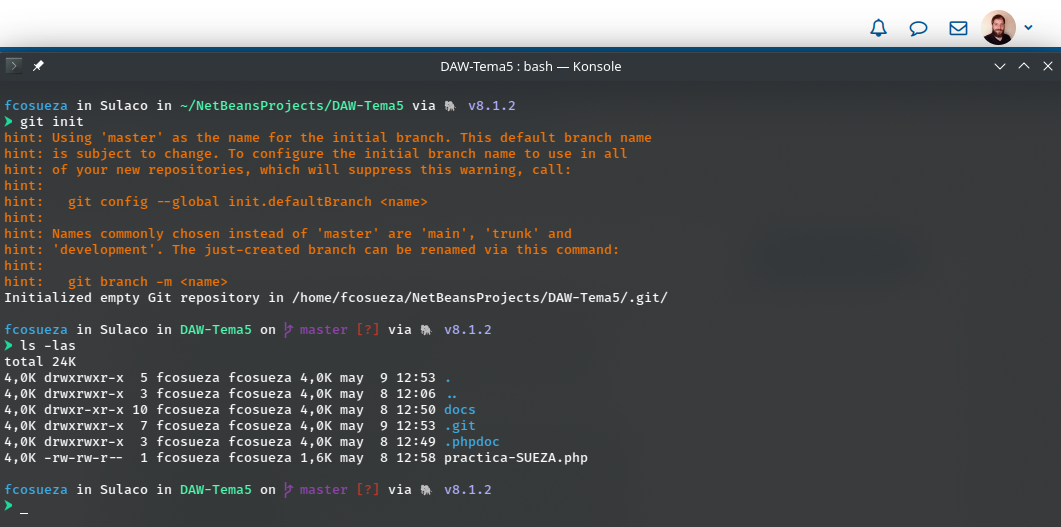
\includegraphics[scale=0.50]{gitInit.png}
    \end{figure}
\end{enumerate}

\subsection{Ejercicio 2.3}
En este apartado que se escogerá el fichero que hemos realizado en el apartado 1.2 y demostrar como funciona git en tal proyecto, por ejemplo subiendo a git todo el proyecto completo y posteriormente es necesario modificar algo para que se detecten los cambios. Es necesario realizarlo con NetBeans. Hay que darse de alta en la url \url{https://github.com/} y crear un repositorio llamado distanciadaw2324 para llevar los ficheros del proyecto php. Demostrarlo con capturas de pantalla.

\subsubsection{Solución}
En este apartado vamos a crear un repositorio en \textbf{GitHub}, y linkearlo con el que hemos creado en el punto anterior, para posteriormente subir todos los archivos del proyecto y realizar alguna modificación.

\begin{enumerate}
    \item En primer lugar vamos a \textbf{crear el repositorio en GitHub}. La creación de la cuenta no se va a incluir en este punto, ya que tenemos una cuenta ya creada y funcional en la plataforma. Para crear el repositorio, desde la pantalla de \textbf{Your Repositories} en Github pulsamos en el botón \textbf{new} y nos aparecerá un formulario donde podremos introducir los datos del repositorio, como podemos ver en la siguiente captura.

    \begin{figure}[H]
        \centering
        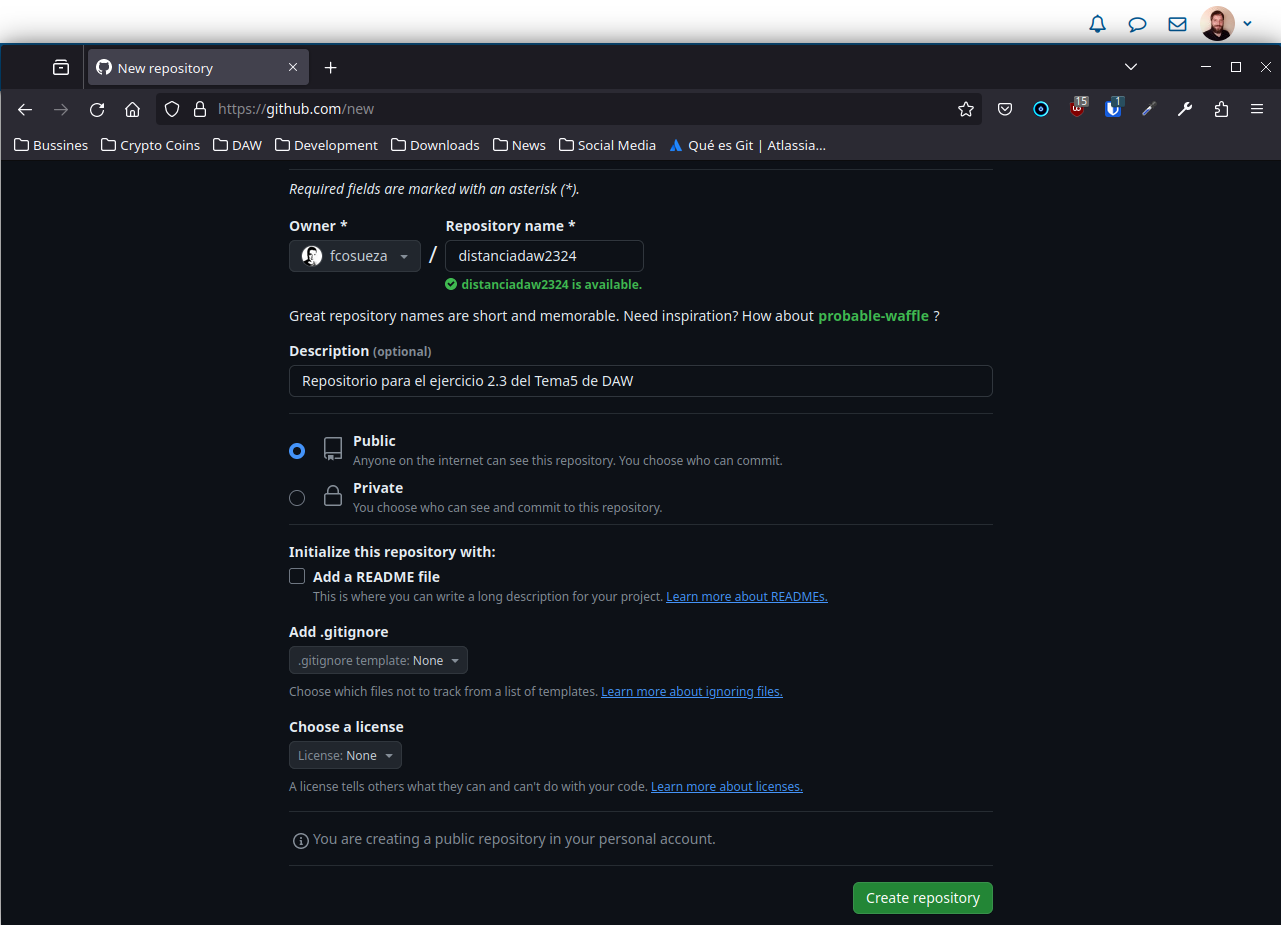
\includegraphics[scale=0.296]{githubNew.png}
    \end{figure}

    \item Una vez que hemos creado el repositorio en Github, vamos a \textbf{añadir} los cambios iniciales del repositorio que creamos en de forma local, mediante los comandos \textbf{\textit{git add -A}}, que añade todos los cambios realizados a la cabecera, en este caso, los archivos que ya estaban en el directorio que hemos creado, y a continuación realizar el commit con \textbf{\textit{git commit -m}}, para añadir finalmente los cambios, como vemos en la siguiente captura.

        \begin{figure}[H]
        \centering
        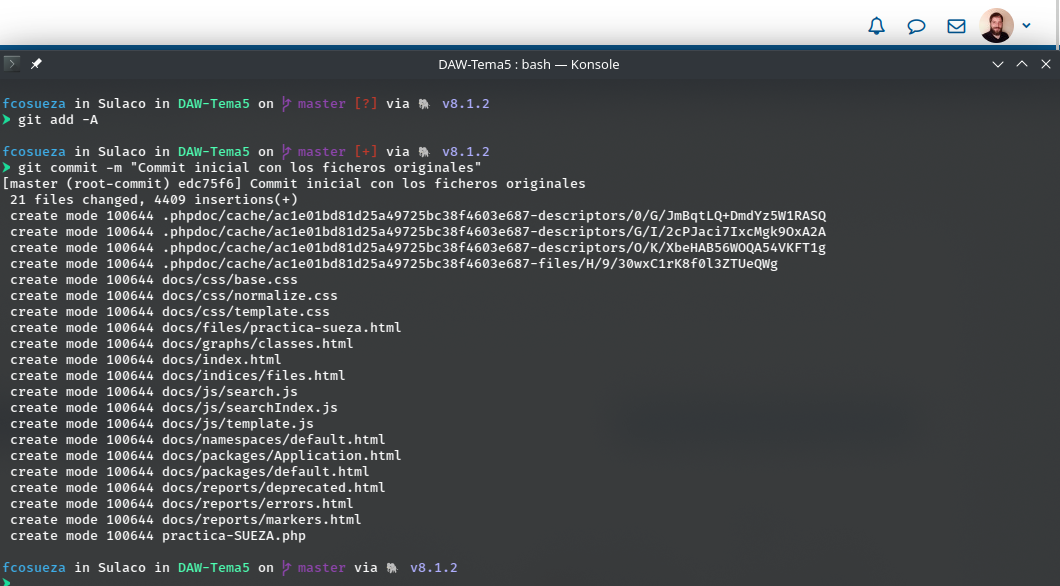
\includegraphics[scale=0.40]{githubLocal.png}
    \end{figure}

    \item Una vez que tenemos nuestro repositorio local al día, vamos a enlazar nuestro repositorio local con el repositorio creado en GitHub. Para ello, vamos a usar el comando \textbf{\textit{git remote add origin git@github.com:fcosueza/distanciadaw2324.git}}, y después los comandos \textbf{\textit{git branch -M main}}, para establecer la rama principal y \textbf{\textit{git push -u origin main}} para subir los cambios al servidor de GitHub.

    \begin{figure}[H]
        \centering
        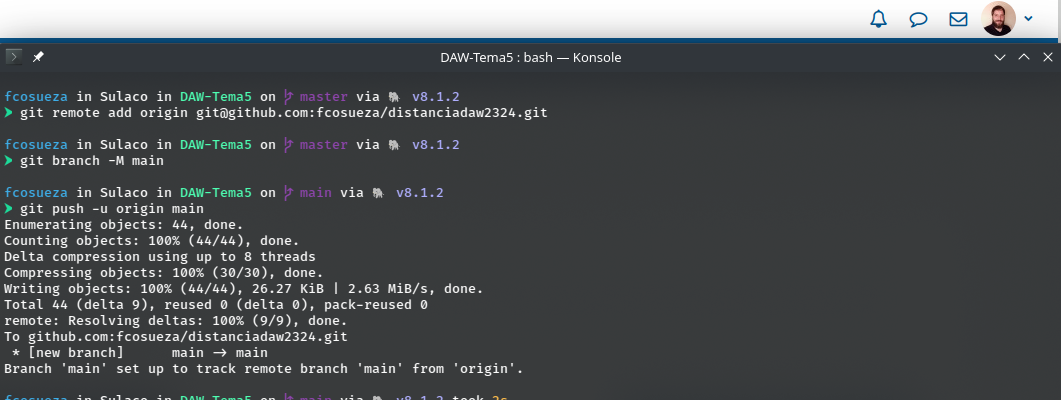
\includegraphics[scale=0.40]{githubLink.png}
    \end{figure}

    Como podemos ver en la siguiente captura, nuestro repositorio de Github se ha actualizado con los archivos que teníamos en nuestro repositorio local.

    \begin{figure}[H]
        \centering
        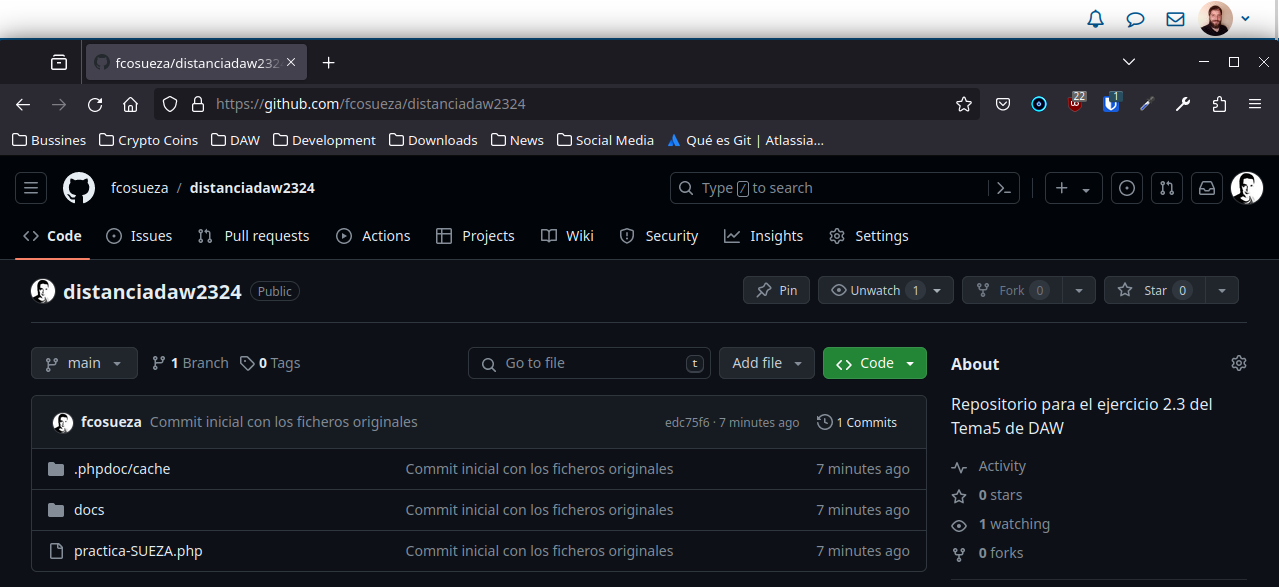
\includegraphics[scale=0.32]{githubUpdate.png}
    \end{figure}

    \item En el siguiente paso, vamos a \textbf{modificar el código} del archivo PHP que tenemos en el repositorio, cambiando el nombre que le pasamos como parámetro a la función \textbf{generarMensaje}, como podemos ver en la siguiente captura.

    \begin{figure}[H]
        \centering
        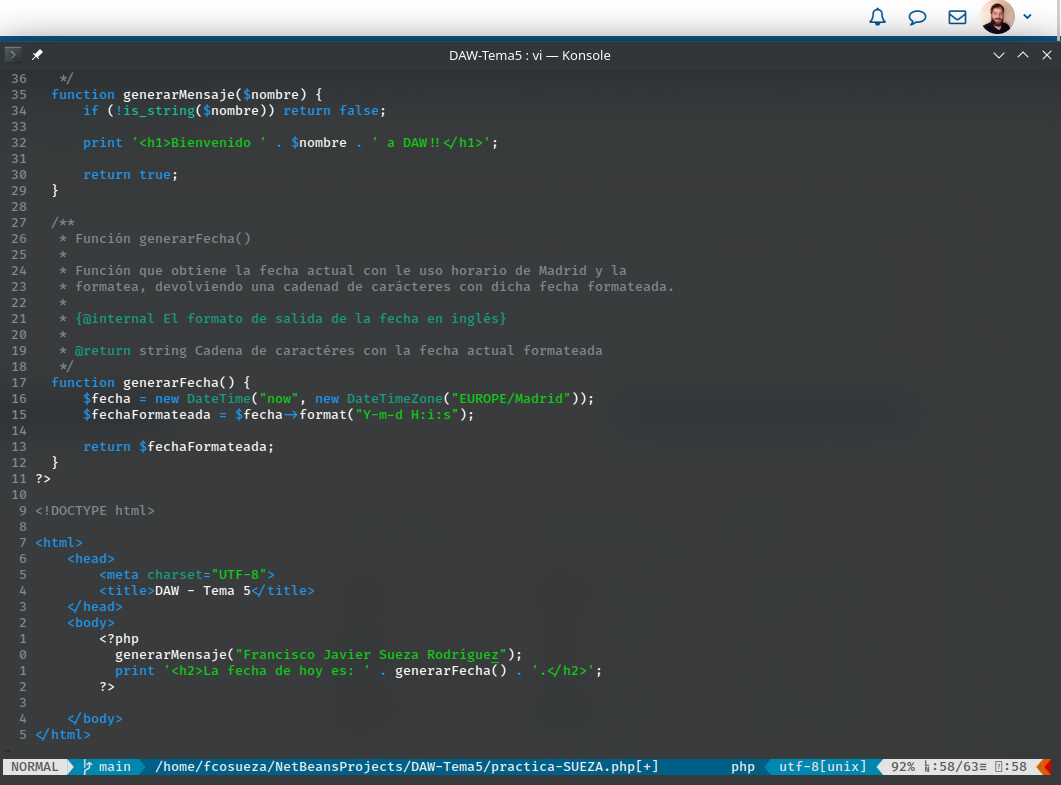
\includegraphics[scale=0.45]{githubChange.png}
    \end{figure}

     \item Ahora debemos actualizar el repositorio, para ellos, usaremos los comandos \textbf{\textit{git add -A}}, para añadir los cambios al stage, el comando \textbf{\textit{git commit -m}} para añadir los cambios al repositorio local, y por último \textbf{git push}, para enviar los cambios al repositorio remoto. En la siguiente captura, vemos la sucesión de comandos.

     Como vemos, no hace falta indicar en el comando push el origen ni la rama ya que hemos establecido por defecto que se suba a la rama master \textbf{main}. Si no fuera el caso, deberíamos especificarlo en cada ejecución del comando push, o en el caso de que tuviéramos varias ramas y quisiéramos actualizar una concreta.

         \begin{figure}[H]
         \centering
         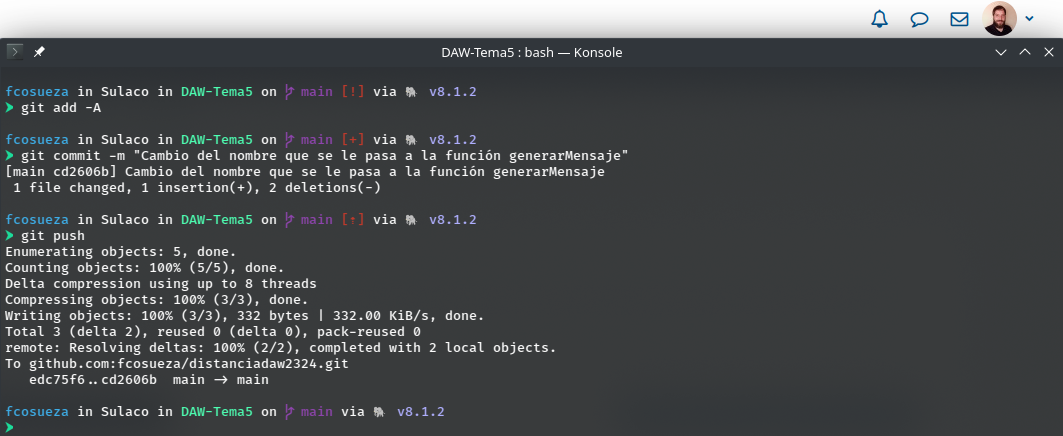
\includegraphics[scale=0.45]{githunPush.png}
     \end{figure}

    \item Una vez realizado esto, nuestro repositorio de GitHub estará actualizado y todos nuestros archivos se habrán modificado. En la siguiente captura podemos ver el historial de modificaciones y los commits que se han realizado en el repositorio.

    \begin{figure}[H]
        \centering
        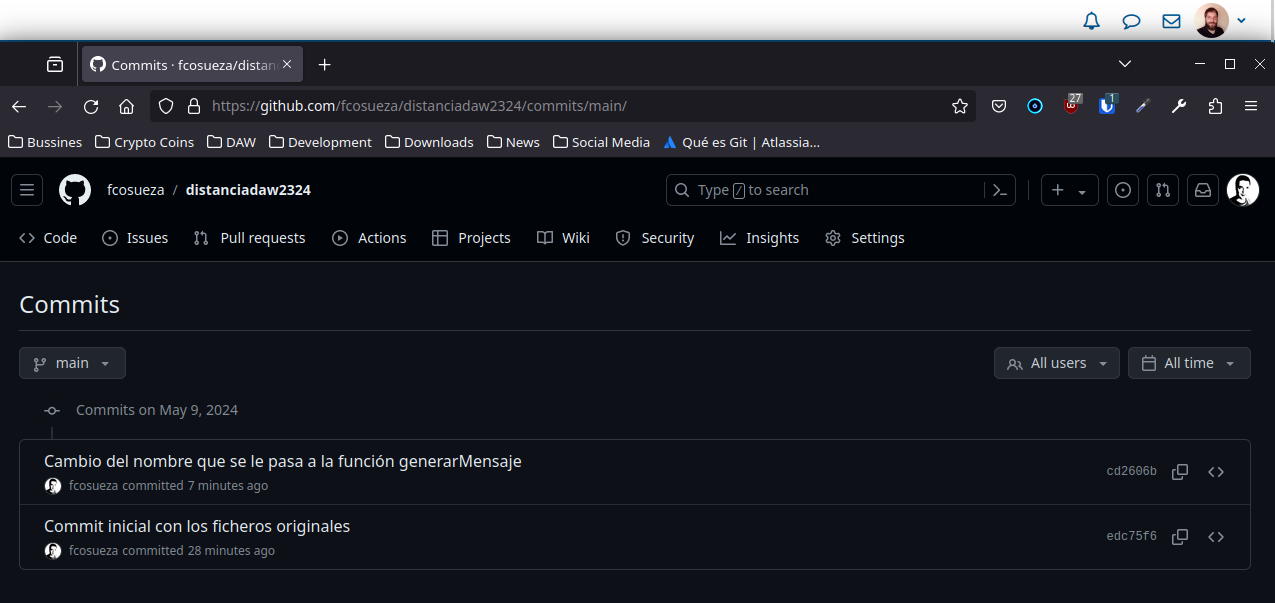
\includegraphics[scale=0.45]{gitCommi.png}
    \end{figure}


    \item Por último, si queremos, podemos visitar el repositorio creado de GitHub en el siguiente enlace: \url{https://github.com/fcosueza/distanciadaw2324}.
\end{enumerate}

%\bibliographystyle{unsrt}

\end{document}